\documentclass[crop,tikz]{standalone}
\usetikzlibrary{backgrounds}
\colorlet{blue}{cyan}
\tikzset{
  inverted/.style = {
    every path/.style = {draw=white,text=white},
    background rectangle/.style={fill},
    show background rectangle
  }
}

\tikzset{>=latex}
\usetikzlibrary{shapes}
\colorlet{gray}{gray!50}

\begin{document}
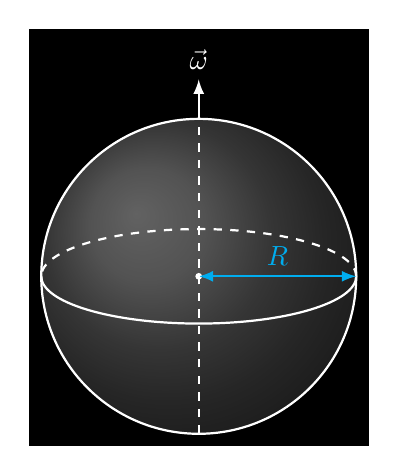
\begin{tikzpicture}[inverted,inverted]
  \shade[ball color = gray, opacity = 0.4] (0,0) circle (2cm);
  \draw[thick] (0,0) circle (2cm);
  \draw[thick] (-2,0) arc (180:360:2 and 0.6);
  \draw[thick,dashed] (2,0) arc (0:180:2 and 0.6);
  \fill[fill=white] (0,0) circle (1pt);
  \draw[<->,blue,thick] (0,0 ) -- node[above]{$R$} (2,0);
  \draw[dashed,thick] (0,-2) -- +(0,4);
  \draw[->,thick] (0,2) -- +(0,0.5) node[above] {$\vec{\omega}$};
\end{tikzpicture}
\end{document}
